Selles peatükis tutvustatakse töö tulemusena valminud rakenduse põhilist funktsionaalsust ning hinnatakse, kuidas see täidab töö alguses püstitatud eesmärke. Lisaks võrreldakse saadud tulemusi ühe olemasoleva lahendusega, analüüsitakse rakendust testinud foneetikauurija tagasisidet ning kirjeldatakse võimalusi edasiarenduseks.

Valminud rakendus on avalikult kättesaadav GitHubi repositooriumis \cite{hrauds_repo}, kus on võimalik rakendus installeerida ja tutvuda koodiga.

\section{Rakenduse funktsionaalsus ja vaated}
Järgnevalt analüüsitakse, kuidas rakenduse vaated ja funktsionaalsus täidavad töö alguses püstitatud kasutusjuhte. Kasutusjuhtude juures on lisatud rakenduse kuvatõmmised, et visualiseerida rakenduse toimimist.

\subsection{Rakenduse kasutajaliidese tutvustus}
Joonisel 1 on esitatud rakenduse põhivaade ja selle komponendid:
\begin{enumerate}
    \item \textbf{Juhtpaneel} (\textit{Control Panel}), kus kasutajal on võimalik salvestusi hallata, valida visualiseerimise tegevus (tunnuste visualiseerimine või sarnasuse visualiseerimine) ning peale tulemuste visualiseerimist andmeid eksportida.
    \item \textbf{Helisalvestuste esitaja} (\textit{Recording Player}) võimaldab helifaili esitamist ning kuvab selle amplituudi visualisatsiooni.
    \item \textbf{Visualiseerimise vaade} (\textit{Visualisation View}): vaates kuvatakse juhtpaneelis tehtud valikute põhjal genereeritud visualisatsioon.
    \item \textbf{Tabelivaade} (\textit{Table View}): vaates kuvatakse visualisatsiooni andmed tabeli kujul.
\end{enumerate}

\begin{figure}[H]
    \centering
    \includegraphics[width=\textwidth]{figures/rakenduse-põhivaate-osad.png}
    \caption{Rakenduse põhivaade ja selle osad.}
    \label{fig:rakenduse-põhivaate-osad}
\end{figure}

\subsection{Kasutusjuhtude analüüs}
Järgnevalt kirjeldatakse, kuidas loodud rakendus täidab funktsionaalsete nõuete kasutusjuhte.

\textbf{GeMAPS tunnuste eraldamine kõnefailidest ja salvestuste töödeldud andmete kustutamine}.
\begin{itemize}
    \item Juhtpaneelis asuv nupp \textit{Manage Recordings} avab salvestuste haldamise akna.
    \item Kasutaja saab \textit{Import Files} nupu abil valida .wav ja .TextGrid faile, mille järel OpenSMILE’i abil eraldatakse GeMAPS tunnused ja salvestatakse MongoDB andmebaasi.
\end{itemize}

Joonisel 2 on esitatud salvestuste halduse aken, kus on näha töödeldud salvestuste nimekiri.
Tulemuseks on, et Kasutaja saab töödelda ja hallata salvestusi. Rakendus kuvab nii õnnestumise- kui ka veateateid, mis on esitatud Lisa 3 joonistel 6 ja 7.
\begin{figure}[H]
    \centering
    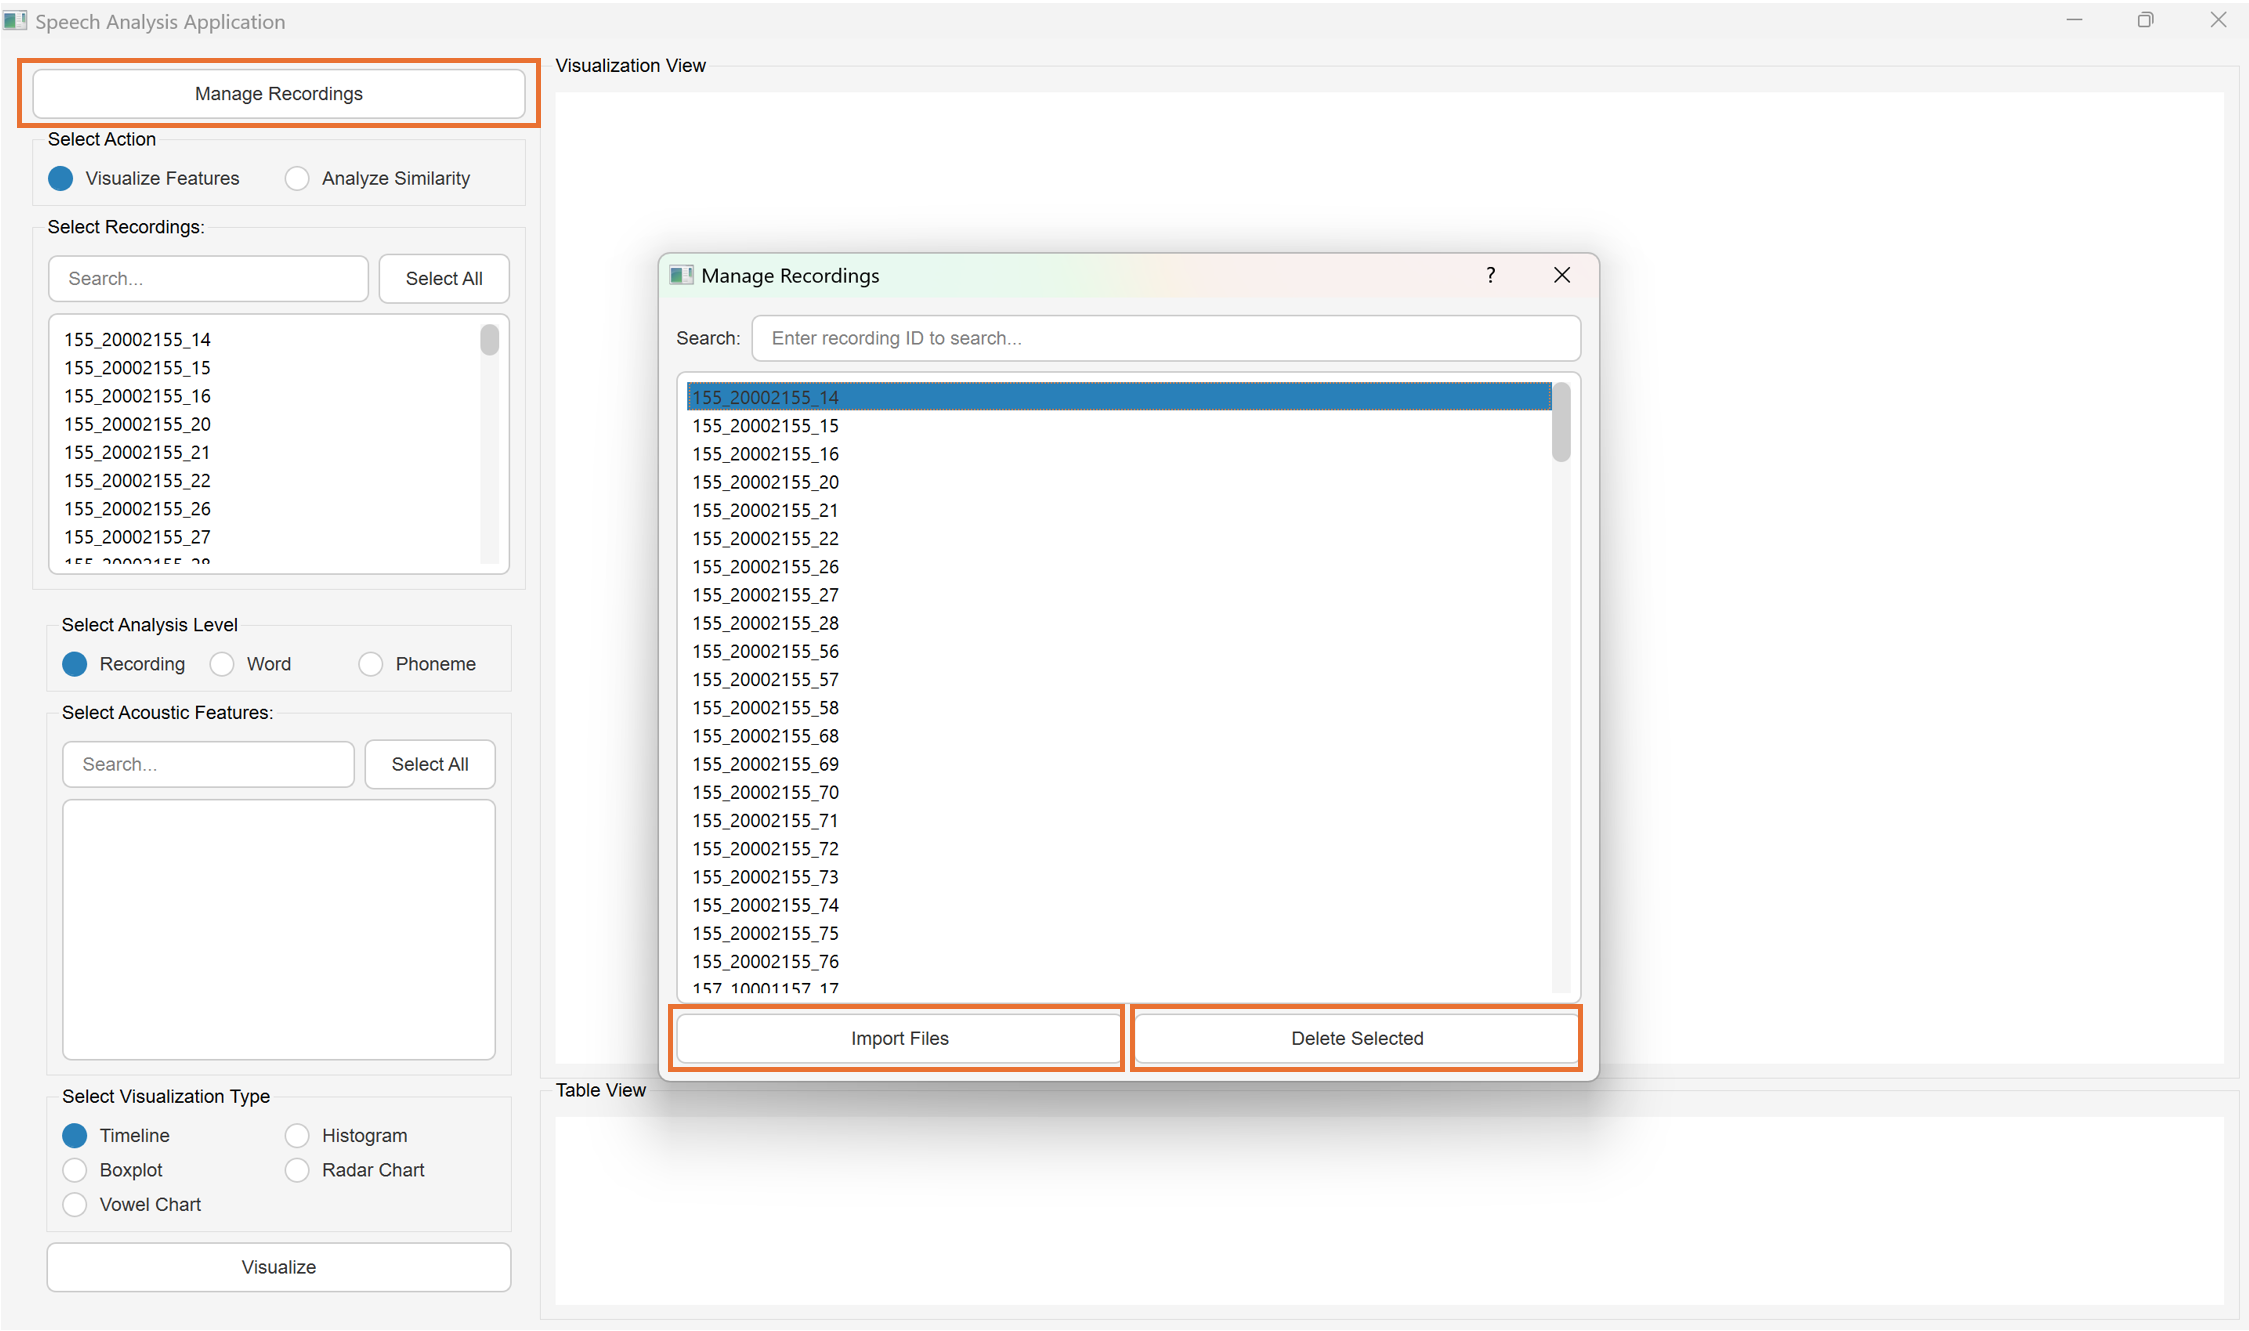
\includegraphics[width=\textwidth]{figures/rakenduse-salvestuste-haldus.png}
    \caption{Rakenduse salvestuste haldus.}
    \label{fig:rakenduse-salvestuste-haldus}
\end{figure}

\textbf{Tunnuste visualiseerimine
}
\begin{itemize}
    \item Visualisatsioonide kuvamiseks kasutaja valib \textit{Visualize Features} valikutest sobivad tunnused.
    \item Valib salvestused (\textit{Select Recordings})
    \item Määrab, kas soovitakse vaadata tunnuseid salvestuse, sõna või foneemi tasandil (\textit{Select Analysis Level}).
    \item Kui valiti foneemi või sõna tasand, tuleb valida ka sõnad või foneemid.
    \item Seejärel valib kasutaja konkreetsed GeMAPS tunnused (\textit{Select Acoustic Feature}s) ning sobiva graafikutüübi (nt ajatelg, karp-, histogramm, radar, vokaalikaart).
    \item Pärast nupule \textit{Visualize} vajutamist, kuvatakse \textit{Visualization View}, kus on: interaktiivne graafik, mille paremas ülanurgas tööriistad (suurendus, pildi eksport jm).
    \item Visualisatsiooni vaate all kuvatakse tabelivaade (\textit{Table View}).
\end{itemize}
Joonisel 3 on näha tunnuse visualiseerimine sõna kohta.
\begin{figure}[H]
    \centering
    \includegraphics[width=\textwidth]{figures/rakenduse-tunnus-sõna-timeline.png}
    \caption{Joondiagrammi näide ühe sõna ja tunnuse visualiseerimisel.}
    \label{fig:rakenduse-tunnus-sõna-timeline.png}
\end{figure}

\textbf{Sarnase kõneleja leidmine}
\begin{itemize}
    \item Kasutaja valib \textit{Analyze Similarity} valiku, määrab salvestused, mida omavahel võrrelda (\textit{Select Recordings}).
    \item See järel Valib ühe (\textit{Target Recording}) salvestuse, millega teisi võrrelda ning sisestab arvu, mitu kõige sarnasemat salvestust soovitakse tulemusena saada (\textit{Number of Similar Items}).
    \item Seejärel valib kasutaja sarnasuse visualiseerimise meetodi: \textit{Cluster Analysis (PCA + KMeans)}, \textit{Feature Similarity Bars} (koosinussarnasus) või \textit{PCA-Based Similarity Bars} (koosinussarnasus PCA ruumis).
    \item Pärast nupuvajutust arvutab rakendus sarnasuse tulemused (nt klasterdamise või koosinussarnasuse), ning kuvatakse \textit{Visualisation View}, kus on: tulpdiagramm, mis näitab salvestuste sarnasuse väärtust või hajuvusdiagramm (klastrite korral), mis eristab klastreid värvidega ning märgib sihtsalvestuse ja kõige sarnasemad salvestused eri sümbolitega.
\end{itemize}

Joonisel 4 on esitatud näide sarnasuse visualiseerimisest PCA ja koosinussarnasuse meetodiga

\begin{figure}[H]
    \centering
    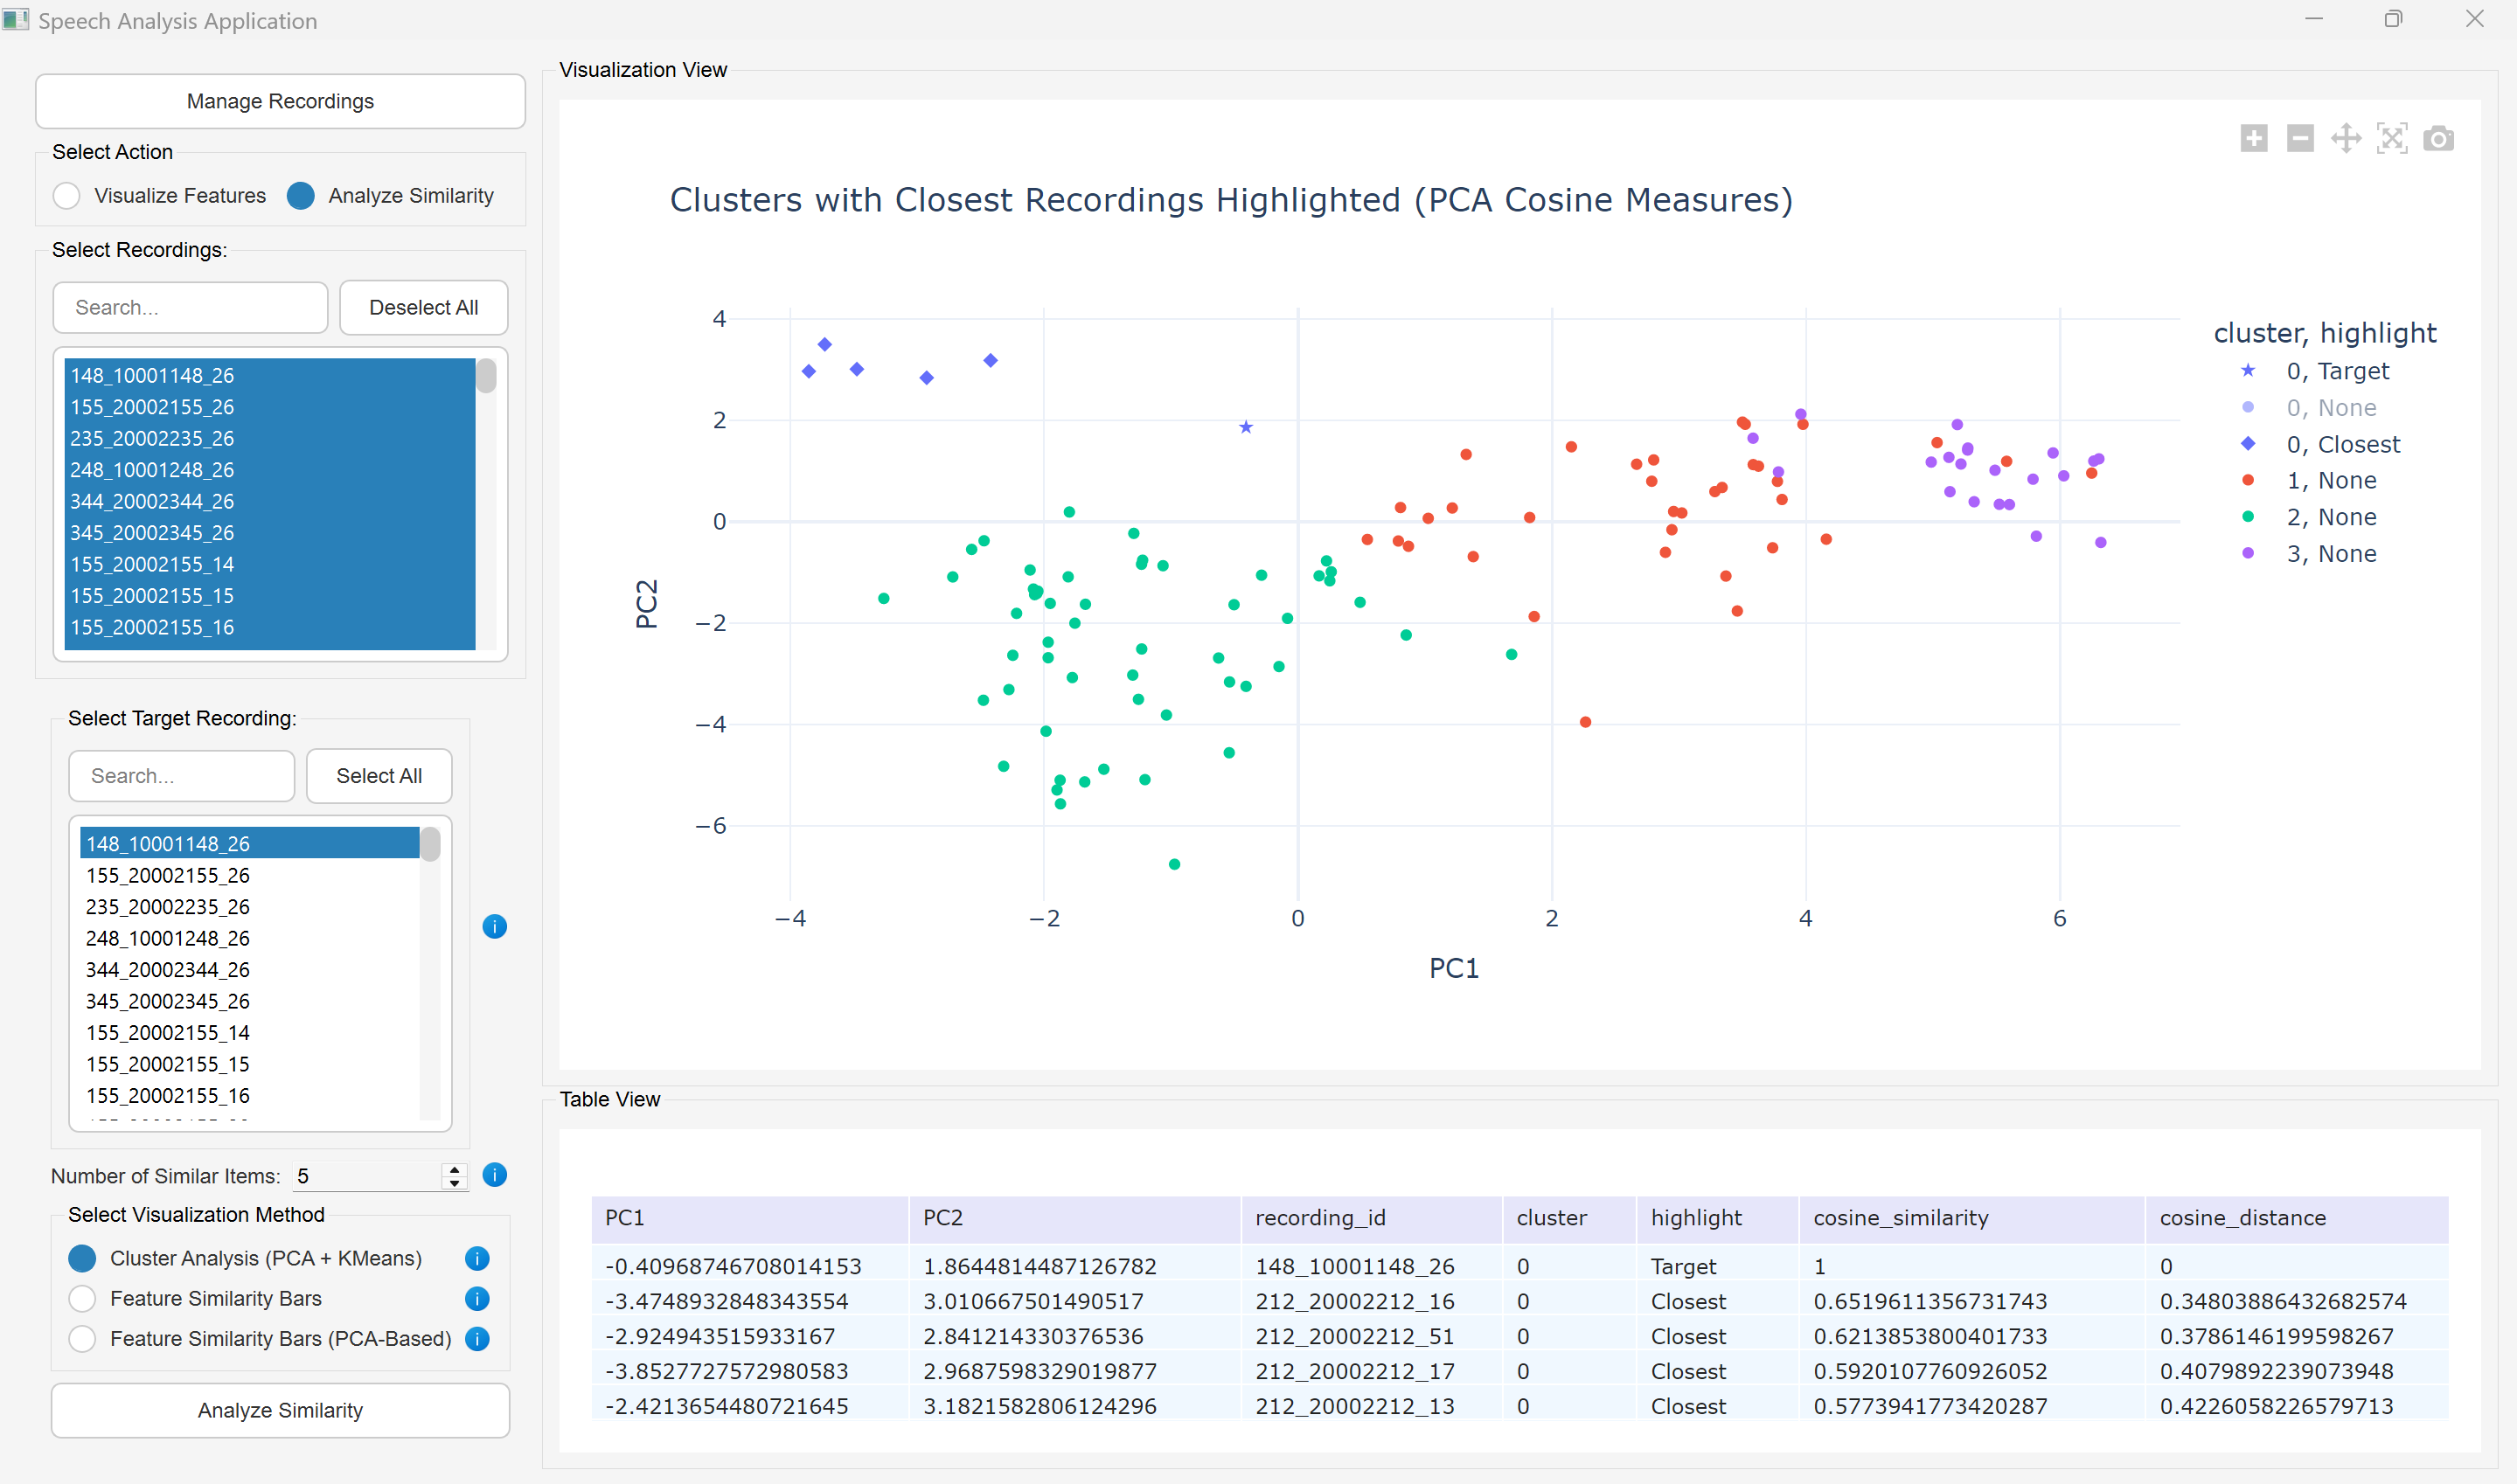
\includegraphics[width=\textwidth]{figures/rakenduse-sarnasus-cluster-closest.png}
    \caption{PCA koosinussarnasuse ja klastrite visualiseerimine hajuvusdiagrammil.}
    \label{fig:rakenduse-sarnasus-cluster-closest}
\end{figure}

\textbf{Helisalvestuse esitamine ja helilaine visualiseerimine}

\begin{itemize}
    \item \textit{Recording Player} sektsioonis kuvatakse rakenduse \textit{data} kaustas asuvad salvestused.
    \item Kasutaja valib faili ning vajutab \textit{Play} nuppu.
    \item Rakendus mängib helisalvestust ning samal ajal kuvatakse helilaine. Mõlemad on kuvatud Joonisel 1.
\end{itemize}

\textbf{Andmete ja visualisatsioonide eksportimine}
\begin{itemize}
    \item Iga valminud graafiku kohal on kaamera märgiga nupp (Plotly sisseehitatud funktsioon). See võimaldab kasutajal salvestada staatilise pildifaili.
    \item Lisaks on juhtpaneelis \textit{Export Graph Data (JSON)} nupp, mis salvestab kasutatud andmed JSON-vormingus. Nupud on nähtaval Joonisel 3.
\end{itemize}

\section{Tulemuse võrdlus olemasoleva lahendusega}
Järgnevalt võrreldakse valminud rakenduse funktsionaalsust Kõneveebi Audiofailide akustiliste omaduste võrdlemise lahendusega (Joonis 5). Kuna see tööriist on alternatiivsetest lahendusest kõige sarnasem oma fookuse, eesmärgi ja funktsionaalsuse poolest. Kuigi Praat või VoiceSauce on palju laiemalt kasutatud akustiliste tunnuste analüüsimisel, on nende fookus ja funktsionaalsus palju laiem ning nad ei keskendu kitsalt eGeMAPS-tunnuste komplektile, nagu Kõneveebi lahendus ja ka loodud rakendus. Seega on sobivam rakendust võrrelda Kõneveebi lahendusega.

\begin{figure}[H]
    \centering
    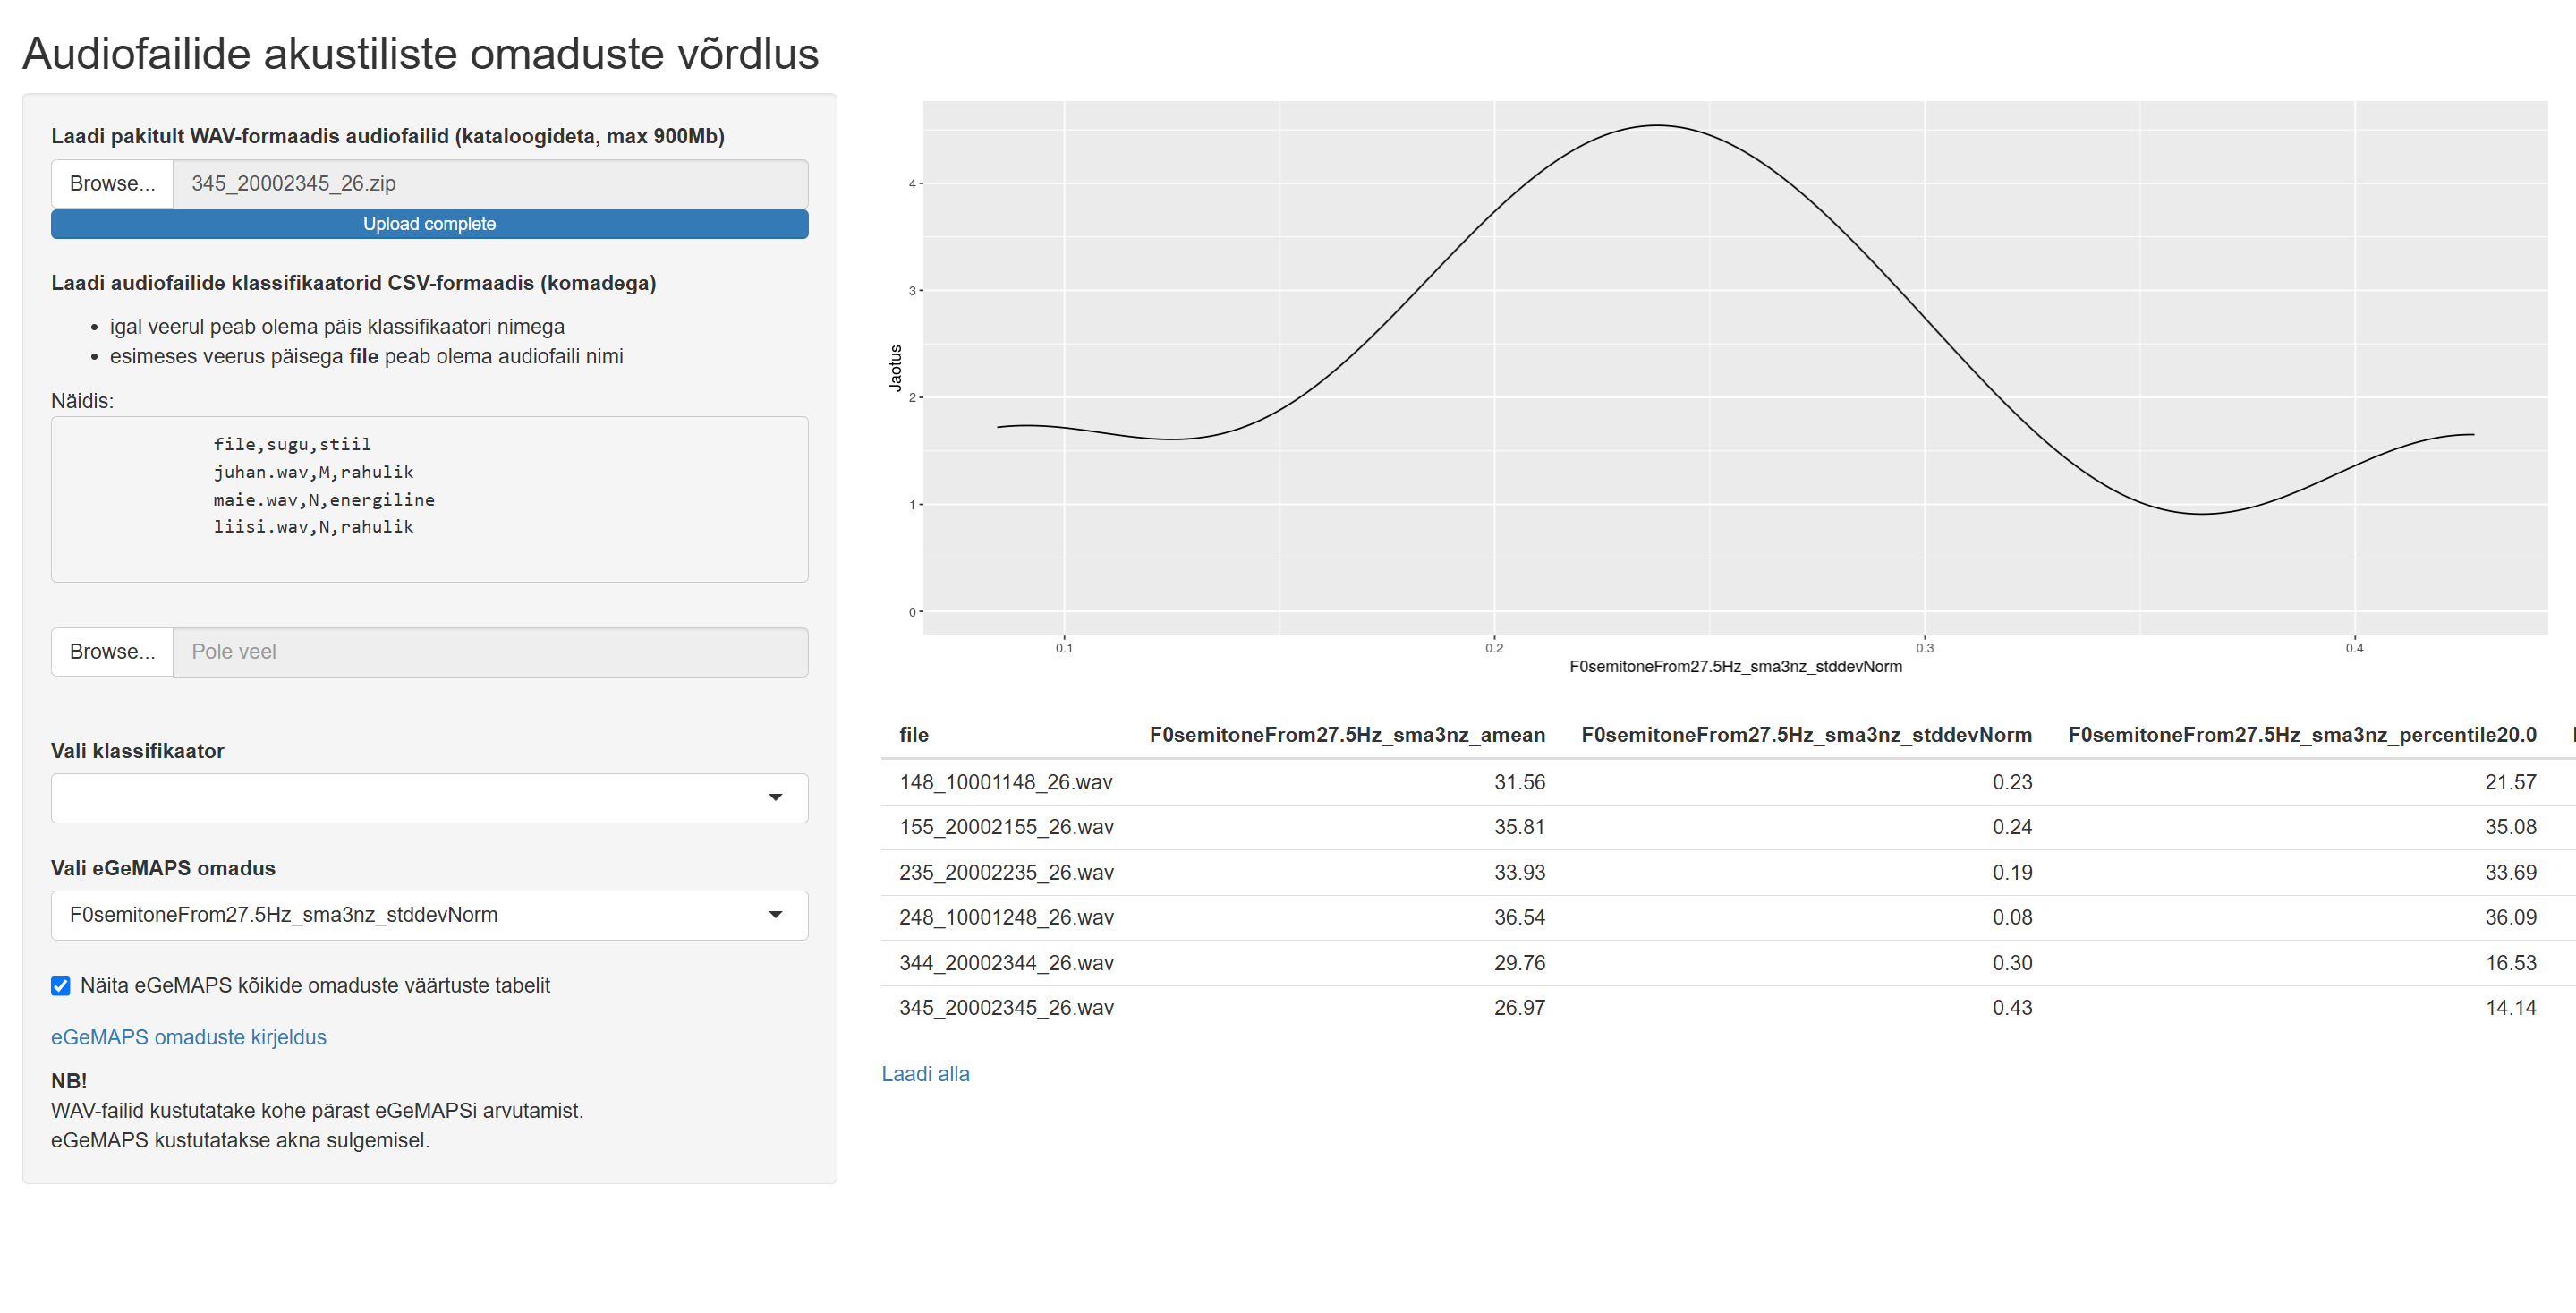
\includegraphics[width=\textwidth]{figures/alt-kõneveeb-põhivaade.png}
    \caption{Kõneveebi Audiofailide akustiliste omaduste võrdlemise rakenduse põhivaade.}
    \label{fig:alt-kõneveeb-põhivaade}
\end{figure}


\begin{longtable}{|p{2.5cm}|p{5.5cm}|p{5.5cm}|}
    \hline
    \textbf{Omadus} & \textbf{Kõneveeb} & \textbf{Loodud rakendus} \\
    \hline
    \endfirsthead
    \hline
    \textbf{Omadus} & \textbf{Kõneveeb} & \textbf{Loodud rakendus} \\
    \hline
    \endhead
    \hline
    \endfoot
    \hline
    \endlastfoot
    
    Tunnuste komplekt &
    Võimaldab analüüsida tervet 88 tunnusega eGeMAPS tunnustekomplekti. &
    Võimaldab analüüsida ainult eGeMAPS v02 LLD komplekti, mis sisaldab üksnes madala taseme deskriptoreid (LLD). \\
    \hline
    
    Rakenduse tüüp &
    Veebirakendus. &
    Installitav töölauarakendus, töötab lokaalselt. \\
    \hline
    
    Kasutajaliides &
    Sarnane põhivaate ülesehitusele nagu loodud rakendusel: juhtpaneel valikutega vasakul ning paremal visualiseerimise ja andmetabeli sektsioonid. &
    Sarnane põhivaate ülesehitusele nagu kõneveebil: juhtpaneel valikutega vasakul ning paremal visualiseerimise ja andmetabeli sektsioonid. \\
    \hline
    
    Erinevate graafikute valik &
    Joondiagramm. &
    Pakub laiemat valikut tunnuste graafikuid, sealhulgas ajatelje diagramm, histogramm, karpdiagramm, radardiagramm, vokaalikaart. Sarnasuse analüüsil on võimalik kasutada hajuv- ja tulpdiagramme. Samuti on graafikud interaktiivsed. \\
    \hline
    
    TexdGridide info kasutamine &
    Ei paku võimalust lugeda ega töödelda TextGrid-failides sisalduvaid ajaintervalle (sõnu, foneeme). Analüüs piirdub salvestuse tasemega. &
    Võimaldab lugeda TextGrid-faili, seostada konkreetsete tunnuste väärtusi sõna või foneemi ajaintervalliga ning seejärel kuvada eraldi vaateid/visualiseeringuid valitud segmentidele. \\
    \hline
    
    Sarnaste salvestuste leidmine &
    Puudub. &
    Võimaldab mitut sarnasuse arvutamise meetodit (klasterdamine, koosinussarnasus, PCA-järgne koosinussarnasus). Visualiseerib tulemused kas tulpdiagrammina (näiteks kõige sarnasemad salvestised) või hajuvusdiagrammil, kus sihtsalvestis ja sarnased salvestised on esile tõstetud. \\
    \hline
    
    Andmete eksport &
    On nupp arvutatud tunnuste andmete allalaadimiseks, kuid see ei toiminud antud töö kirjutamise ajal. &
    Toetab andmete eksporti JSON faili ja pildifaili kujul. \\
    \hline
    
    Andmete haldus &
    Üleslaetud failid ja arvutatud tunnused kustutatakse seansi lõpus. Failide maht on piiratud (kuni 900 MB) ja tulemusi ei salvestata. &
    Kasutab MongoDB andmebaasi analüüsi andmete hoidmiseks. \\
    \hline

\end{longtable}

Kokkuvõttes on Kõneveebi rakendusel ja loodud rakendusel sarnane põhifookus, kuid veidi erinev ulatus. Kõneveeb on kindlasti mugav ja kiirem, kuna see ei vaja eraldi installeerimist ja seadistamist. Kuid käesolev rakendus on laiema funktsionaalsusega ning sobib paremini mahukamaks analüüsiks, kus on vaja erinevaid visualiseerimise meetodeid, analüüsitulemuste salvestamist ja sarnasuse analüüsi.

\section{Tagasiside}
Rakenduse valideerimiseks küsiti tagasisidet ühelt foneetikauurijalt, kellele saadeti rakenduse installeritav versioon koos kasutusjuhendiga ja tagasiside küsimustega, mis on esitatud Lisas 4.

\textbf{Rakenduse graafikute arusaadavus ja kasulikkus}. Testija tagaside oli, et rakenduses loodud graafikud olid üldiselt arusaadavad ning märgiti, et need võiksid olla mugavad kiireks analüüsiks. Kõige kasulikumaks visualisatsiooniks peeti vokaalikaarti.

\textbf{Tehnilised probleemid ja tõrked}.
Tagasiside põhjal ei märgatud rakenduse kasutamise ajal tehnilisi probleeme ega tõrkeid

\textbf{Kasutajasõbralikkuse hinnang}.
Kasutajasõbralikkuse ja mugavuse osas anti rakendusele hinnang 3 skaalal 1-5, kus 1="väga mugav" ja 5="väga ebamugav". Kuigi rakendus ei olnud kasutaja arvates väga ebamugav, mainiti, et mõned klikkimisega seotud iseärasused vajasid harjumist.

Näiteks tekitas segadust, et histogrammi visualisatsiooni valik muutub mitte-aktiivseks, kui on valitud korraga üle kahe tunnuse ja salvestuse korraga. See oli tahtlik piirang, et vältida olukordi, kus liiga paljude tunnuste ja salvestuste samaaegne kuvamine ühel graafikul muudaks tulemused raskesti loetavaks. Selle piirangu oleks pidanud kasutajale arusaadavamaks tegema näiteks teavituste või infonuppude abil, nagu tehti paljude rakenduse teiste funktsioonide puhu, kuid kahjuks jäid need selle piirangu jaoks lisamata.

\section{Võimalused edasiarenduseks}
Rakendusel on palju võimalusi edasiarendusteks. Järgmiselt tuuakse välja mõned võimalused, mis tulid esile peale arenduse lõppu:
\begin{itemize}
    \item Võimaldada erinevate GeMAPS tunnustekomplektide arvutamine
    \item Võimaldada erinevate normaliseerimismeetodite rakendamine ja mitte rakendamine, et kasutajal oleks rohkem kontrolli andmete visualiseerimisel. Näiteks vokaalikaardi puhul normaliseeritakse väärtused Lobanov meetodiga ja ei ole võimalust teisi meetodeid kasutada või väärtused normaliseerimata jätta.
    \item Kasutajaliidese mugavdamine: näiteks menüüs võiks olla rohkem ruumi tunnuste ja salvestuste valimiseks
    \item Sarnasuse analüüsi valideerimine, rohkem meetodeid sarnaste salvestuste leidmiseks
    \item Andmete mahu probleemi lahendamine: kui andmete hulk kasvab, muutub rakendus aeglasemaks
    \item Muuta rakendus lihtsamini installeeritavaks, et kasutaja ei peaks MongoDB andmebaasi seadistama.
\end{itemize}

Lisaks tõi foneetikauurija tagasisides esile järgmised soovitused:
\begin{itemize}
    \item Lisada funktsioon helifailide lõikamiseks.
    \item Luua võimalus esitada helifaile otse failide valiku menüüst.
    \item Kuvada rakenduses rohkem arvandmeid.
\end{itemize}
